\chapter[Processing Text]{Processing Text} 
\label{chapter:nlptext}
\begin{center}
%{\Large\textit{You just do it like that and shit works\ldots -I. Langmore}}
\end{center}
\vspace{0.2in}

%\section{History} 
%\label{text:history} 
%Something about where this comes from\ldots 

\section{A Quick Introduction}
%\begin{itemize}
%  \item Regular expressions
%  \item Text processing
%  \item Python NLTK library
%  \item Tokenization
%  \item Corpus
%  \item Python Pattern library
%\end{itemize}


With the influx of information during the last decade came a vast, ever growing, volume of \T{unstructured data}. An accepted definition of \T{unstructured data} is information that does not have a pre-defined data model or does not fit well into relational tables (if you have not seen relational database or tables, think of collection of python pandas data frames or similar containers). A large part of this category is taken up by text, which is what we will focus on in this chapter. 


From news publication, websites, emails, old document scans, social media the data world today is filled with text and many times it is up to the data scientist to extract useful information or usable signals. Much of this work falls into the realm of data processing and uses a variety of techniques from UNIX \t{regular expressions} to \T{natural language processing}. The following three are common examples: 

\begin{itemize}
    \item Text Classification: lets say you start with a collection of newspaper articles and the task is to properly place each into the appropriate news category. The task would be to first extract useful features from the text - these could be simply words, or nouns, or phrases - and then use these features to build a model.
    \item Web scraping: your task it to write a program that will crawl a number of websites, process the text and extract common themes, topics, or sentiment levels.
    \item Social media trends: your task is to analyze the reaction of twitter users to particular news events and to identifying those which are currently ``trending'' or have the potential of going ``viral.'' 
\end{itemize}

\section{Regular Expressions}
\label{regex}

Regular expressions \cite{WPRegEx} are an incredibly power tool for patter matching in text. 
They originated from automata and formal language theory of the 1950's and later, being integrated in \textit{Unix ed}, \textit{grep} 
and \textit{awk} programs, became an indispensable part of the Unix environment. The power of regular expressions comes from their flexibility and syntactical 
compactness; they form a language in their own right, which takes a bit of getting used to. However, with 
a little practice you become attuned to the internal logic and intelligent design. 

Python incorporates the regular expressions toolbox in a standard library called \textit{re}. You can find most of the 
information you will need at \\ http://docs.python.org/2/library/re.html. The library allows for added 
functionality on top of returning search patterns, such as boolean match function, replacement, etc

\subsection{Basic Concepts}

The easiest way to understand regular expressions is to begin using them, so lets start with an example. We are going to 
take a simple string of characters and extract some information from them. Hopefully you will have a terminal open
and can following along. 

\begin{minted}{python}
import re
myString = "<I am going to show 2 or maybe 10 examples
of using regular expressions.>"
re.findall(r"[a-zA-Z0-9]", mystring)    
\end{minted}

returns a list of every alphanumeric character that appears in the string above, i.e. we get a list of 57 characters from 'I' to 
s. As you can probably guess the code inside the parentheses simply asks for any character that is either a letter (any case) 
or a number. If we would like to include the period in this list, we can simply add it to the list of characters we are 
interested in.

\begin{minted}{python}
re.findall(r"[a-zA-Z0-9.]", s)    
\end{minted}

If we are interested in words, numbers included, and not just the individual characters we can include a "+" at the end of the expression, which is special as it 
matches one or more characters in the preceding regular expression, i.e.

\begin{minted}{python}
re.findall(r"[a-zA-Z0-9]+", s)    
\end{minted}

returns the list l = [`I',
 `am',
 `going',
 `to',
 `show',
 `2',
 `or',
 `maybe',
 `10',
 `examples',
 `of',
 `using',
 `regular',
 `expressions']. 


 Of course, typing character ranges explicitly as we did above can become a bit tedious, so there are special shorthand symbols to make life easier. For example
 we could have returned the above list by evoking

 \begin{minted}{python}
re.findall(r"\w+", s)    
\end{minted}

so now we know that `[a-zA-Z0-9]' = ``\textbackslash w'' in \textit{RE}. If we want all the symbols include the angled parentheses at the beginning and end of the string, we could 
call


 \begin{minted}{python}
re.findall(r".", s).    
\end{minted}

If are looking for all instances where a period appear, we could return that by calling

\begin{minted}{python}
re.findall(r"\.", s).    
\end{minted}

Hence, we have learned a few things about regular expression syntax: we have ways of matching certain characters, or ranges of characters; there 
is shorthand notation for common searches; there are special or "wild-card" characters, and ways of escaping those special characters (names by
calling "\textbackslash"). 

Now it's time to look at things a bit more formally. 



\subsection{Unix Command line and regular expressions}

We have already quite a bit about Unix command-line functions and utilities. You can think of Unix in terms of grammatical language structure, where:

\begin{itemize}
    \item commands like \textit{ls}, \textit{ls}, \textit{man} are thought of as verbs
    \item the objects, files, data to operate on as nouns
    \item shell operators, such as | or >, as conjunctions
\end{itemize}

so what we are missing now are some adjectives, and we can think of \textit{regular expressions} as filling this gap. We've already seen some regular expressions so lets look at a table of the core syntax. 

\begin{center}
    \begin{tabular}{c|l}
        \hline
        . & Match any character \\ \hline
        \^{} & Match the start of a string \\ \hline
        \$ & Match the end of a string or just before the newline character \\ \hline
            \textbackslash d & Match any decimal digit \\ \hline
            \textbackslash D &  Match any single non-digit character \\ \hline
            \textbackslash w & Match any single alphanumeric character  \\ \hline   
            [A-Z] & Match any of uppercase A to Z. \\ \hline
           ? &	Match zero or one occurrence of the preceding regular expression \\ \hline
            * &	Match zero or more occurrence of the preceding regular expression \\ \hline
            + &	Match one or more occurrences of the preceding regular expression. \\ \hline
            \{n\} &	Match exactly n occurrences of the preceding regular expression.\\ \hline
            \{m,n\} &	Match from m to n repetitions of the preceding regular expression \\ \hline 
            
        
    \end{tabular}
\end{center}

Lets look at some examples. Suppose you have a file \textit{people.txt} which contains the names of all the people in the class. It looks like:

\begin{minted}{bash}

Kate Student
Jake Student
Ian Professor
Emily Student
Daniel Professor
Sam Student
Chang Professor
Paul Student
\end{minted}

If you want something trivial such as retrieving all lines with professor names you can type

\begin{minted}{bash}
    grep Professor people.txt
\end{minted}

or even 

\begin{minted}{bash}
    grep Pr people.txt
\end{minted}

both of which return

\begin{minted}{bash}
Ian Professor
Daniel Professor
Chang Professor
\end{minted}

However, suppose you would like to do something slightly less trivial such as finding all people in the class whose name starts with the letter `P.' If you try something like

\begin{minted}{bash}
    grep P people.txt
\end{minted}

this will return 


\begin{minted}{bash}
Ian Professor
Daniel Professor
Chang Professor
Paul Student
\end{minted}


i.e. every line with a capital `P' in it. You can use regular expression to help out; do so you on some systems you will need to invoke the `E' flag 

\begin{minted}{bash}
    grep -E "^P" people.txt
\end{minted}

which will return 

\begin{minted}{bash}
Paul Student
\end{minted}

as desired. 


For another, perhaps more natural, example suppose you are a systems administrator and you need to find all login related processes as well as all processes corresponding to a certain user.  You can type

\begin{minted}{bash}
ps -e | grep -E "login|daniel"
\end{minted}

which will return the appropriate PID, time and command executed.


Lets look at a more interesting example. Suppose you have a big file and you would like to extract all lines which constitute a valid date, where a valid date is of the \textit{yyyy-mm-dd} format, between 1900-01-01 and 2099-12-31, with a choice of separators. Hence, we would accept character substrings \textit{2000-01-15} and \textit{2000/01/15}, but not \textit{2000/01-15}. The regular expression that would do this for you is



\begin{minted}{bash}
(19|20)\d\d[-/](0[1-9]|1[012])[-/](0[1-9]|[12][0-9]|3[01])
\end{minted}

This is a bit convoluted so lets fo through it. The first thing to notice is that there are three main groups
defined by brackers $()$; these are:

\begin{minted}{bash}
 (19|20)
 (0[1-9]|1[012])
 (0[1-9]|[12][0-9]|3[01])
\end{minted}

The first part just makes sure that you are looking for a string that starts with 19 or 20. The second group makes sure that you that the month starts with either a 0 or 1 and contunes with the appropriate digit, and similiar for the dates. In addition, we have a '\^{}' to signify that we are looking at the start of a line, then \d signifies we are looking for a number between 0 and 9, the $[- /.]$ which allows either a dash or a backslash. 

Note, there are some issues with this particular regular expression since it will match dates like \textit{2003-02-31}, but also it will match dates like \textit{2004/04-12} which you wanted to exclude. We'll see ways to get around this. 


\subsection{Finite State Automata and PCRE}

There are a number of different implementation of regular expressions, resulting in varied flexibility and performance. The ``original'' framework is modelled on \textit{finite state machines} \cite{WPFSM} making for a very fast and efficient approach. The complexity of finite automata implementation, referred to as \textit{re2}, is O(n) where n is the size of the input, but it does have its limitation. The main reason is that a finite state machine does not ``remember'' how it arrived at a given state, which prevents from evaluating a latter piece of a regular expression based on an earlier one. 

For example, suppose we have the following simple regex:

\begin{minted}{bash}
    "[ab]c+d"
\end{minted}

The machine will first check to see if there is ``a'' or ``d'' in the string, then whether it followed by one or more ``c"'s and then a ``d." Now by the time it makes to say ``d" it doesn't remember why it made it there, how many ``c"'s it encountered, or that this was preceded by an "a." You can visualize the situation with the following diagram

%\begin{displaymath}
%    \xymatrix{
%        \bullet \ar@/^/[r]
%        \ar@/_/@{.>}[r] &
%        \bullet }
%\end{displaymath}

This is precisely the limitation which prevented us from distinguishing between valid dates, i.e. those with either all "-" or "/" as separators, above.  One solutions is to extend the regular expression syntax to include \textit{backreferences}. The \textit{PCRE}, or \textit{Perl Compatible Regular Expressions}, implementation, which is what python \textit{RE} module was originally based on. However, matching regular expressions with backreference is an NP-hard problem.

\begin{figure}
  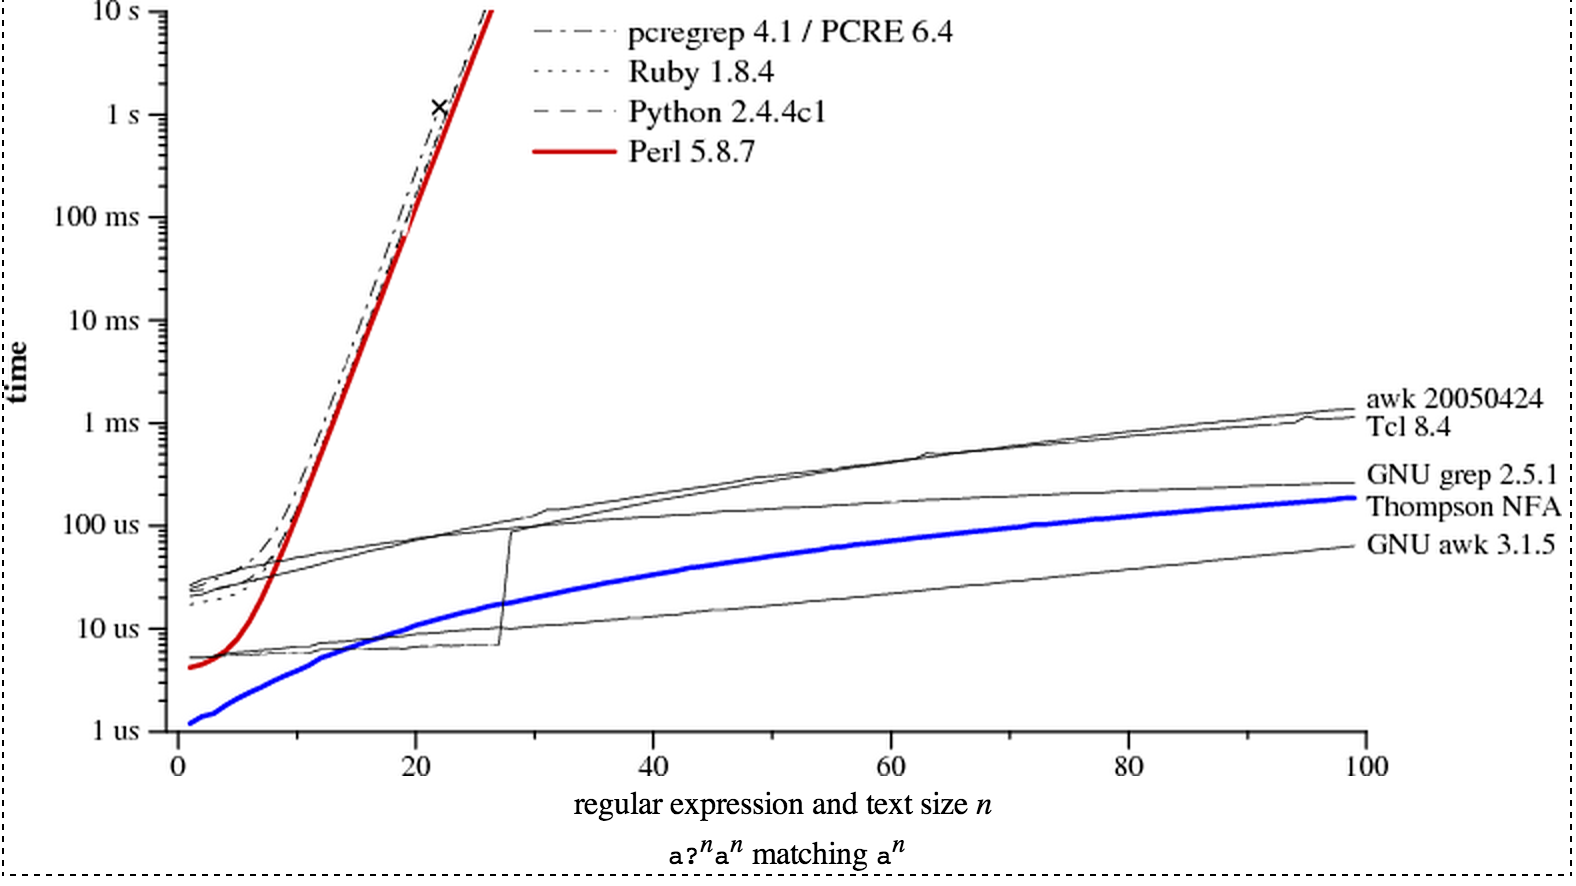
\includegraphics[width=\textwidth]{../images/RegExAlg}
  \caption{Regular Expression Implementation Time Comparison (see \cite{RegExComp} for more details)}
  \label{regex:regexALg}
\end{figure}






\subsection{Backreference} 

To mitigate the limitation of standard regular expression as described above, \textit{backreferences} were introduced. You can find these in the python \textit{RE} module as well as when calling grep with the -E flag (for \textit extended).

The basic syntax is quite simple, and is evoked by writing \textbackslash N to refer to the N'th group. If we refer back to the valid dates example from above we would replace the second set of [-/]'s with a backreference to first, ensuring a consistent match.

\begin{minted}{bash}
(19|20)\d\d([-/])(0[1-9]|1[012])\2(0[1-9]|[12][0-9]|3[01])
\end{minted}

Note that we are calling \textbackslash 2, because the first group is (19|20).

Of course, even backreferences don't solve all your problems, but they are big help. If you were trying to match something a bit more flexible such as balanced parentheses you would need a counter or just some additional scripting.


\begin{exercise}
    Use the python regular expression library to write a script that matches all lines in a file with balanced parentheses.
\end{exercise}


\section{Python RE Module}


The python regex library is an amazing tool that combines the power of regular expression, with backreference, and the flexibility of the python language. most of the syntax is inherited from unix, as above, but there are a few additions. 

There is also a large array of methods that come with the library, and a selection of the more noted is the following:

\begin{itemize}

    \item The findall function:

        
\begin{minted}{python}
re.findall(pattern, myString)
\end{minted}

        which returns all non-overlapping patterns in a string. For example,

\begin{minted}{python}
re.findall(r"\d+", "My number is 212-333-3333, and you can call 5-6pm")
\end{minted}

will return 

\begin{minted}{python}
["212", "333", "3333", "5", "6"]
\end{minted}




    \item The search function:

\begin{minted}{python}
re.search(pattern, myString)
\end{minted}

        which scans through a string and returns a \textit{re.MatchObject}, which always has a boolean value but also a number of methods. 
        For example, 

\begin{minted}{python}
myString = "My number is 212-333-3333, and you can call 5-6pm")
s = re.search(r"\d+", myString)
if s:
    print s.group(0)
\end{minted}

will print the number 212, since it is the first pattern match in the string. You can also do much more intelligent things with groups. For example, suppose you wan to check for the existence of a phone number and time and, if possible, return both. The following expression will do exactly that. 

\begin{minted}{python}
myString = "My number is 212-333-3333, and you can call 5-6pm")
s = re.search(r"(\d{3}-\d{3}-\d{4}).+(\d{1}-\d{1})(am|pm)", myString)
if s:
    print "this is the whole match:", s.group(0)
    print "this is the number:", s.group(1)
    print "this is the time:", s.group(2)
    print "this is the meridiem:", s.group(3) 
\end{minted}


Note, you can do a lot niftier things with groups in python's \textit{RE} module, such as attributing keys. For example,

\begin{minted}{python}
s = re.search(r"(?P\<number\>\d{3}-\d{3}-\d{4}).+(?P\<time\>\d{1}-\d{1})(?P\<ampm\>am|pm)", "My number is 212-333-3333, and you can call 5-6pm")
if s:
    print "this is the number:", s.group("number")
    print "this is the time:", s.group("time")
    print "this is the meridiem:", s.group("ampm")
\end{minted}




    \begin{digression*}[Difference between match and search]
        The only difference between re.match() and re.search() is the fact that match looks for patterns at the beginning of a string and search anywhere within. You can turn a search into a match function by appending a \^{} to the beginning of the patter at hand. 

    \end{digression*}


    \item The sub and split function. 

    
        These substitute a given found regex pattern with a string, or split on a given pattern. The basic syntax is

\begin{minted}{python}
    re.split(pattern, string)
    re.sub(patter, stringSub, string)
\end{minted}


\end{itemize}


\vspace{.5 in}

\newpage


\begin{digression*}[Why the "r?"]
    As you might have noticed there are two ways to enter a regular expression into a python \textit{RE} method, either in quotes or with a "r" appended to the front. The r invokes python's raw string notation and the reason for is that the use of backslash in regex to as an `escape' character, i.e. to allow special/wild characters to be used for a literal match, collides with python's use or a backslash for the same purpose in string literals. Hence, to match a backslash in a string using \textit{RE} you would have to write 

\begin{minted}{python}
re.findall("\\\\", myString),
\end{minted}

i.e. two backslashes to escape the special meaning in regex and two to escape it in python strings. If this were left so you can imagine a complete rigmarole, but luckily we can invoke the raw string notation and arrive at the same function with more sane syntax:

\begin{minted}{python}
re.findall(r"\\", myString)
\end{minted}


\end{digression*}



The python \textit{RE} library is very rich and incredibly powerful. We invite you to explore more on the module website \url{http://docs.python.org/2/library/re.html#re.MatchObject}.

\vspace{.5 in}


\begin{digression*}[fnmatch]

    In case you are wondering if there is a way to run unix shell-style wildcards from within python the answer is via the \textit{fnmatch} module. 
    For example, if you would like to print all filenames in a given directory with .txt extension, i.e. the equivalent of 

\begin{minted}{bash}
ls *.txt
\end{minted}

you can run

import fnmatch
import os

\begin{minted}{python}
for file in os.listdir('.'):
    if fnmatch.fnmatch(file, '*.txt'):
        print file
\end{minted}

Or if you would like to convert *.txt to it's regex equivalent

\begin{minted}{python}
regex = fnmatch.translate('*.txt')
\end{minted}

There are other modules that are great for handling paths and file extensions, such as glob, but the above can be useful from time to time. 


\end{digression*}


%\section{Text Processing}
%\label{textProc}


\section{The Python NLTK Library}
\label{nltk}

\subsection{The NLTK Corpus and Some Fun things to do}
\label{sub:nltk_corpus}

The NLTK library contains a large corpus, ranging from \textit{Moby Dick} to a collection of presidential inaugural addresses, which can be used for exploration of library, model development, etc/ 
You can see the work by typing 

\begin{minted}{python}
from nltk.book import *
texts()
\end{minted}


and explore individuals nltk.text objects by their designated text number. For example "text1" is nltk.text object containing 
\textit{Moby Dick}. Object method can be explored as usual by typing "text1. + tab" (if you are using ipython or and IDLE with tab 
completion). 

\begin{minted}{python}
from nltk.book import *
text.name
\end{minted}

\noindent returns "Moby Dick by Herman Melville 1851" and

\begin{minted}{python}
from nltk.book import *
text1.similar(`whale')
\end{minted}

\noindent returns 

\vspace{0.1in}
\noindent\textit{"ship boat sea time captain deck man pequod world other whales air crew
head water line thing side way body"}
\vspace{0.1in}


\noindent which are not surprisingly the words that appear in a similar context to "whale."



The frequency distribution of words is common to consider when looking at given text. This can lead to some interesting 
statistics which can be used for analysis, classification or text comparison. The \textit{NLTK} library provides 
an instance for such exploration. The following commands will call \textit{FreqDist}, return the first 10 items (in decreasing 
count order), return the count for "whale," as well as its frequency. 

\begin{minted}{python}
freqDist = nltk.FreqDist(text1)
freqDist.items()[:10]
freqDist[`whale']
freqDist.freq(`whale')
\end{minted}

There is an additional set of functionalities that come along with \textit{nltk.FreqDist}, such as max, plot, hapaxes (
words that appear only once), and many others which are helpful for exploration. 

Aside from the additions methods that come along with it, \textit{FreqDist} is really a sort and count operation and as 
useful exercise we challenge you to reproduce it with the python \textit{groupby} function from the \textit{itertools} 
library. 


In addition, you can do some fun things like generate random text, based on a trigram language model. For example,


\begin{minted}{python}
from nltk.book import *
text1
text1.generate()
\end{minted}

\noindent generates a random text (default length=100). If you want to generate text based on your own input, which is say of type \textit{str},
you first should coerce input into an \textit{nltk.text.Text} object, i.e. 


\begin{minted}{python}
import nltk
myNltkOText = nltk.text.Text(myStringText)
myNltkText.generate()
\end{minted}

will do the trick. 



some more stuff\ldots.

 


































